\chapter{Node Merging} \label{nodemerging}
	This chapter explains the process of node merging and the VF2 algorithm in detail.

\section{Node Merging Implementation}
In graph transformation, rules are applied on the host graph and the resulting graphs are represented as nodes of a tree. When the application of a rule gives a new graph (node), it needs to be compared with the existing tree nodes. If that node exists already, an edge is added to that node, otherwise, a new node is created. The corresponding code listing can be seen below.

\begin{lstlisting}[language = Java,frame = single]
 for(E rule: rules){
 V newNode = ruleExecutor.execute(node, rule)
 if(newNode != null) {
 /* For all the older nodes in the tree check if it has any match*/
 for(V oldNode:tree.getVertices()){  
        if(nodeComparator.compare(oldNode, newNode)){
	            /* If yes then just add an edge to the existing node */
            Integer edgeId = new Integer(tree.getEdgeCount());
     	    edgeIdToRuleMap.put(edgeId, rule);
    	    tree.addEdge(edgeId, node, oldNode, EdgeType.DIRECTED);
            flag = true;
            break;
        }
    }
 /* If this is a unique graph, create a new node and add it to the tree*/
	   if(!flag){
		    Integer edgeId = new Integer(tree.getEdgeCount()); 
    		edgeIdToRuleMap.put(edgeId, rule);	
	    	tree.addVertex(newNode);
		    tree.addEdge(edgeId, node, newNode, EdgeType.DIRECTED);
        }
    }
}
\end{lstlisting}

\section{Graph Matching}
Two graphs are said to be isomorphic if they have the vertices connected in the same way. Formally, two graphs $G$ and $H$ with graph vertices $V_n =\{1,2,...,n\}$ are said to be isomorphic if there is a permutation $p$ of $V_n$ such that $\{u,v\}$ is in the set of graph
edges $E(G)$ iff $\{p(u),p(v)\}$ is in the set of graph edges $E(H)$ \cite{iso1}.

Exact graph matching or graph isomorphism problem is the computational problem of determining whether two finite graphs are isomorphic. The importance of Graph isomorphism algorithms is very high in multiple fields, such as electronic design automation, chemistry and molecular biology etc.

\subsection{Complexity}
Besides its practical importance, the graph isomorphism problem is a curiosity in computational complexity theory as it one of a
very small number of problems belonging to NP, neither known to be solvable in polynomial time nor NP-complete. At the same time, isomorphism
for many special classes of graphs can be solved in polynomial time and in practice, graph isomorphism can often be solved efficiently \cite{iso2}.
This is a special case of the subgraph isomorphism problem, which is known to be NP-complete. However Laszlo Babai has claimed that the 
Graph Isomorphism can be solved in quasipolynomial time. Quantities which are exponential in some power of a logarithm are called “quasipolynomial” \cite{iso3}.

\subsection{Negative checks}
Before going into the algorithm, negative checks can be performed to avoid the graph matching algorithm and yield faster results.
\begin{enumerate}
\item \texttt{Vertex number equivalence:} The number of vertices should be equal

\item \texttt{Edge Count equivalence:} The sum of the edges should be equal

\item \texttt{Edge order check:} This is one of the important checks because when the graphs don't change much, the edge and vertices numbers may not change. Therefore, sorting the edge arrays and comparing them will give good candidates for the matching algorithm.
\end{enumerate}

\section{VF2 Algorithm}
Algorithms such as Ullman, NAUTY and VF2 can be used to solve the graph isomorphism problem. The VF2 algorithm is one of the fastest algorithms for graphs containing many vertices. The software VFLib and the VF2 algorithm are good starting points for writing the custom implementation. 

The VFLib defines a single interface (state) that a variety of subgraph isomorphism matchers can implement in order for it to work interchangeably. The challenges faced during this implementation  were firstly, to understand the intricate VF2 algorithm and secondly, customizing the algorithm to the current problem. One of the ways to understand any graph matching algorithm is to understand the commonalities among all of the approaches currently used . 

A note on the terminology: In graph comparison one graph will be compared to another, can be denoted as graph1 and graph2 or source graph and target graph. 

The commonalities among all graph matching algorithms are:\cite{ric}
\begin{itemize}
\item \texttt{Recursion:} Any implementation typically has a method that calls itself

\item\texttt{State accumulation:} The recursive method gradually builds up a map of nodes from source graph to target graph, one pair of nodes at a time. Sometime it fails, so it needs to go back to last successful match (backtrack). When it succeeds and needs to report success.

\item \texttt{Mapping:} The implementation typically uses an internal map to keep track of what it's done. So getting mapped nodes is easy.
\end{itemize}
 
\begin{figure}
\centerline{
\includegraphics[width=1.0\columnwidth]{figures/vf2_image.png}
}
\caption{VF2 algorithm }
\label{vf2}
\end{figure}

The basic idea behind the VF2 algorithm is that it tries to find the mapping of vertices between two graphs. 
This process of finding the mapping function can be suitably
described by \textit{State Space Representation (SSR)} \cite{vf2}.
Each state $s$ of the matching process can be associated to a partial mapping solution $M(s)$, which contains only subset of the complete mapping. A transition from a generic states to a successor state $s'$, represents the addition of a pair of matched nodes to partial mapping associated to s in the SSR. The algorithm explores the search graph in the SSR according to a depth-first search strategy. 

In figure \ref{vf2}, the Match(s) procedure plays the role of recursive function, while $s$ and $s'$ play the dual role of state accumulators and feature comparators. $P(s)$ represents the set of candidates to be added to state $s$. A set of feasibility rules can be defined to check the consistency condition. These rules can be both syntactic(depend only on the structure of the graph) and semantic (depend on the attributes of nodes and edges).

\subsection{Tracing of VF2 algorithm}

This section explains the tracing process of the VF2 algorithm. Consider two simple graphs $g1$ and $g2$ (Figure \ref{tikz1}) and assume that node $1$ is equivalent to $a$, $2$ is equivalent to $b$ and so on, both semantically and syntactically (color property). We have a candidate list (all possible mappings) and a $map$, which has the partial mappings from g1 and g2. Whenever the $map$ size is equal to number of vertices in the graph, we stop the algorithm and return success.

\texttt{Successful match:}\\

 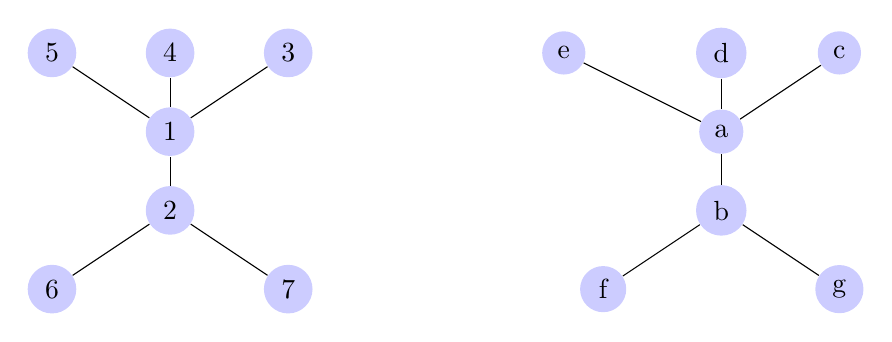
\begin{tikzpicture} 
[scale=.5,auto=left,every node/.style={circle,fill=blue!20}]
  	\node (n5) at (1,10) {5};
    \node (n4) at (4,10)  {4};
    \node (n3) at (7,10)  {3};
    \node (n1) at (4,8)   {1};
    \node (n2) at (4,6)  {2};
    \node (n6) at (1,4)  {6};
    \node (n7) at (7,4)  {7};

  \foreach \from/\to in {n5/n1,n4/n1,n3/n1,n2/n1,n2/n6, n2/n7}
    \draw (\from) -- (\to);

  	\node (n5) at (14,10) {e};
    \node (n4) at (18,10)  {d};
    \node (n3) at (21,10)  {c};
    \node (n1) at (18,8)   {a};
    \node (n2) at (18,6)  {b};
    \node (n6) at (15,4)  {f};
    \node (n7) at (21,4)  {g};
  
  \foreach \from/\to in {n5/n1,n4/n1,n3/n1,n2/n1,n2/n6, n2/n7}
    \draw (\from) -- (\to);

 \end{tikzpicture}
 \captionof{figure}{Graph g1 (left) and Graph g2 (right) for comparison}
    \label{tikz1}
%\end{left}

Before the start of the algorithm, $map$ is $null$. The algorithm consists of the following steps:

\begin{itemize}
\item \texttt{Step 1:} Create initial state that has all the possible vertex combinations as a candidate list.\\ 
Candidate list for initial match is:  $\{ (1,a) (1,b) (1,c)... (7,g)\}$ \\
We remove a candidate from the candidate list and check for feasibility. The feasibility rules checks if the current candidate can be added to the $map$.\\

\item \texttt{Step 2:} We get a match for (1,a). We add this to $map$ and create a new state with a new candidate list (combinations of neighbors of 1 and a).\\
$map$ = \{(1,a)\} \\
candidate list = \{(5,e) (5,d)(5,b)..... (2,b)\}\\
Then, the match procedure is called on this new state. 

\item \texttt{Step 3:} A match is found between (5,e). This is added to $map$ and a new candidate list is generated and the match procedure is called. 
$map$ = \{(1,a) (5,e)\}\\
candidate list = \{ \}.

\item \texttt{Step 4:} Now the candidate list is empty, so now it backtracks. In backtracking, it checks if the head(5) and all of its neighbors are mapped (in this case, it is true) and returns to the previous step. Now, the state is denoted as:\\ 
$map$ = \{(1,a) (5,e)\}\\
candidate list = \{(4,d)(4,b)..... (2,b)\} --> Notice that (5,e) (5,d) etc have been removed

\item \texttt{Step 5:} Check the feasibility of next candidate and continue until the map size is equal to number of vertices.\\ 
.\\
.\\
.\\
\item {\texttt{Step n:}} The size of $map$ is equal to the number of vertices. Return true.
\end{itemize}

\texttt{Unsuccessful match:}\\\\
 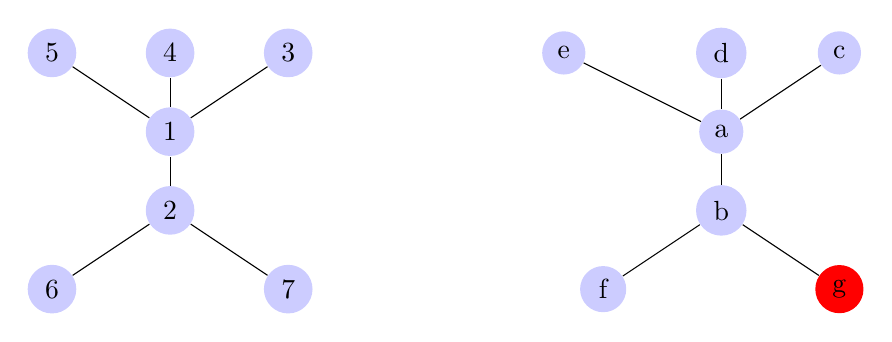
\begin{tikzpicture} 
[scale=.5,auto=left,every node/.style={circle,fill=blue!20}]
  	\node (n5) at (1,10) {5};
    \node (n4) at (4,10)  {4};
    \node (n3) at (7,10)  {3};
    \node (n1) at (4,8)   {1};
    \node (n2) at (4,6)  {2};
    \node (n6) at (1,4)  {6};
    \node (n7) at (7,4)  {7};

  \foreach \from/\to in {n5/n1,n4/n1,n3/n1,n2/n1,n2/n6, n2/n7}
    \draw (\from) -- (\to);

  	\node (n5) at (14,10) {e};
    \node (n4) at (18,10)  {d};
    \node (n3) at (21,10)  {c};
    \node (n1) at (18,8)   {a};
    \node (n2) at (18,6)  {b};
    \node (n6) at (15,4)  {f};
    \node[fill = red] (n7) at (21,4)  {g};
  
  \foreach \from/\to in {n5/n1,n4/n1,n3/n1,n2/n1,n2/n6, n2/n7}
    \draw (\from) -- (\to);

 \end{tikzpicture}
 \captionof{figure}{Graph g1  (on the left) and Graph g2(on the right) for comparison}
    \label{tikz}

Now, we have two graphs of the same structure but differing in their node properties. The algorithm runs like this. 
Consider we are in a step where the state looks like this, \\
$map$ = \{ (1,a) (2,b) (6,f)\}\\
candidate list  = \{(7,g)\} \\

At this stage, it removes (7,g) from the candidate list to check for feasibility, but it does not match. It then goes back to the previous step ($2$) and checks if all of its neighbors are mapped. Since nodes $7$ and $g$ are not mapped, the algorithm removes 2 and 6 from the mapping and continues with a different part of the graph where it hopes to find the mapping for $b$. When all possible mappings are exhausted, the algorithm returns false. 

\subsection{Improvements to original algorithm}
A few improvements or changes were done to the original algorithm in order to suit for the current graphs. In the current graphs, we have strict node properties, and node properties should match for the graphs to be equal. 

\begin{itemize}
\item \texttt{Change 1: Using matchedNodeCandidates data structure}
\begin{lstlisting}[language = Java,frame = single]
/*  holds the matched source nodes for each node in the target graph */
public Map<EObject, Set<EObject>> matchedNodeCandidates; 
\end{lstlisting}

Before we start the match procedure, we check if a node from the target graph has any matching node in the source graph. If we do not find at least one match, then the matching process can be stopped.

\item \texttt{Change 2: Selecting the start node}\\
The traditional implementation takes the combination of all possible vertices as the initial candidate list. An improvement made to select a unique node candidate as the start node, which is a node having only one matching between source and target graph.

\item \texttt{Change 3: Backtracking}\\
Our program spends a lot of time backtracking, as this is an essential part to find the appropriate match. But, if the necessary checks are not carried out, this can increase the time significantly. If the head is mapped, that is when we have mapped the candidate and all of its neighbors successfully, then we safely go back to the previous step keeping the current mappings. If these conditions fail, then we remove the last mapped candidate and continue the process.

There is one more important check that needs to be carried out to avoid backtracking to a great extent. Since we have \textit{matchedNodeCandidates}, we can effectively determine if the removal of the last matched candidate and continuing the algorithm would yield the result. To remove the last successful match, there should be different vertices to match these candidate vertices. If we don't have any, then backtracking should be stopped, since there can be no vertices which can be mapped to the candidate vertices.

\end{itemize}

\subsection{Implementation}
In the present work, the basic idea of the VF2 algorithm is preserved, while a lot of modifications were made for the practical purpose.
 
\begin{figure}
\centerline{
\includegraphics[width=0.6\columnwidth]{figures/folder.png}
}
\caption{folder structure}
\label{folder}
\end{figure}

Figure \ref{folder} shows the VF2 implementation in the current project.
As seen in the figure \ref{folder}
IsomorphismTester.java is an interface which defines a function which will be implemented in VF2IsomorphismTester.java.
\\
\\

\begin{lstlisting}[language = Java,frame = single]
public interface IsomorphismTester {
/*
 * Return true if the graphs are Isomorphic
 */
boolean areIsomorphic(Graph<EObject, EClass> g1, Graph<EObject, EClass> g2);
}
\end{lstlisting}

State.java is an interface, which corresponds to the state s of the VF2 algorithm. VF2State.java implements State interface. 
\\

Some of the data structures used are,

\begin{lstlisting}[language = Java,frame = single]
/*possible candidates to add it to state */
private ArrayList<Pair<EObject>> candidates; 
	
private ArrayList<EObject> sourcePath; // Holds matched vertices of source
private ArrayList<EObject> targetPath; // Holds matched vertices of target

\end{lstlisting}

VF2IsomorphismTester.java defines match procedure along with implementing areIsomorphic() function. 

\begin{lstlisting}[language = Java,frame = single]
private boolean match(State s) {
		if(s.isGoal()){
			maps.add(s.getVetexMapping());
			return true;
		}
		if(s.isDead())
			return false;
		
		boolean found = false;		
		while(!found && s.hasNextCandidate()){
			Pair<EObject> candidate = s.nextCandidate();
					
			if(s.isFeasiblePair(candidate)) {
				State nextState = s.nextState(candidate);
						
				found = match(nextState);
			
				if(nextState.backtrack()){			
				}
				else{
					return false;
				}
			}
	}
		return found;
}
\end{lstlisting}

s.isGoal() returns true if all vertices are mapped.\\
s.isDead() returns false when vertex number mismatch happens. 

After the necessary checks, it choses the initial candidate as our start node pair and checks for feasibility of the candidate. And if it is a feasible candidate, a next state is created, with the current candidate added to $map$.
And the match procedure is called on the next state. Once we run out of candidates, the match function returns and checks for backtracking. If it is a successful backtrack, the matching continues. Otherwise, match terminates by returning false. \\

\texttt{s.nextState():}
\texttt{s.nextState} returns a new VF2State by copying all the previous state values and adding the current candidate to the state. Additionally, it loads the new candidates for matching, which are the combinations of neighbors of previous candidates. 

\section{Results}
Most of the comparisons were eliminated by negative checks and the individual node matching step. For a graph having 315 nodes, the time taken for a successful match is 17 seconds and for an unsuccessful match is 12.5 seconds. This is a good result considering the setup time.

Figure \ref{result} shows the resulting graph obtained by node merge. 
\begin{figure}
 \centerline{
 \includegraphics[width=1.0\columnwidth]{figures/result.png}
 }
 \caption{Resultant graph after node merge \cite{vf2}}
 \label{result}
 \end{figure}
 


